\section{Vincoli}
Durante lo sviluppo del progetto l'azienda non ha imposto particolari vincoli di tipo architetturale, ma sono emersi alcuni vincoli tecnologici, progettuali, metodologici e temporali che influenzano le scelte di implementazione. 
\subsection{Vincoli tecnologici}
Dal punto di vista tecnologico, l'azienda ha imposto l'utilizzo di \textbf{\textit{Python}} (v.3.12.10) come linguaggio di programmazione. Questa scelta è dettata non solo dalla sua versatilità e dalla disponibilità di numerose librerie utili allo sviluppo, ma anche perché rappresenta uno dei linguaggi più diffusi nell'ambito della \textit{cybersecurity}, oltre a essere quello su cui l'azienda possiede maggiore esperienza interna. Per la gestione e la visualizzazione dei dati si è optato per lo \textit{stack \textbf{TIG}}, composto da \textit{Telegraf} (v.1.24), \textit{InfluxDB} (v.2.7) e \textit{Grafana} (v.9.5.6), preferito al più diffuso \textit{stack} \gls{elk} per la sua leggerezza e per la maggiore aderenza ai requisiti del progetto. Anche le modalità di comunicazione tra i diversi componenti sono soggette a vincoli: il tutor ha infatti imposto l'uso del protocollo \textit{\textbf{MQTT}}, particolarmente adatto allo scambio di dati in tempo reale con un consumo ridotto di risorse. Al contrario, non erano previsti vincoli riguardo ai servizi vulnerabili da esporre all'interno del sistema \textit{honeypot}, lasciando piena libertà di scelta in base alle esigenze di implementazione. 
Sul piano progettuale, il tutor aziendale ha stabilito che il sistema dovesse includere un \textit{logger} interno. Questo vincolo ha avuto un impatto diretto sulla progettazione complessiva, in quanto ha reso necessaria l'integrazione di meccanismi di \textit{logging} fin dalle fasi iniziali, in modo da facilitare il \textit{debugging} durante lo sviluppo.
\begin{figure}[H]
    \centering
    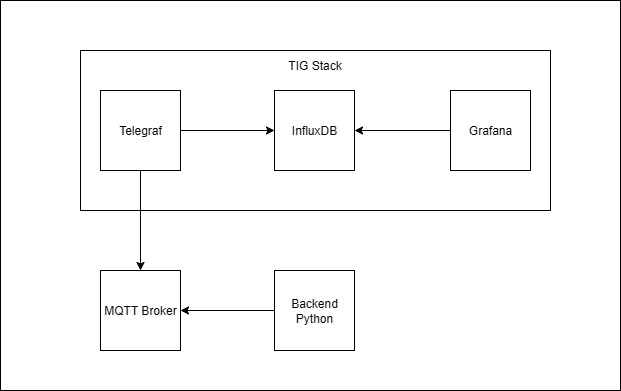
\includegraphics[alt={Schema MQTT-TIG}, width=\columnwidth]{img/mqtt-tig.png}
    \caption{Schema di esempio dell'integrazione tra protocollo \textit{MQTT} e \textit{stack} \textit{TIG}.}
    \label{fig:mqtt-tig}
\end{figure}
\subsection{Vincoli metodologici}
Per quanto concerne la metodologia, il progetto si è sviluppato in quattro fasi principali, che hanno guidato sia la pianificazione sia l'esecuzione: 
\begin{itemize}
    \item \textbf{Fase 1 (Setup dell'ambiente)}: predisposizione di un contesto sicuro e, al tempo stesso, sufficientemente vulnerabile per ospitare \textit{honeypot} e servizi di interesse;
    \item \textbf{Fase 2 (Sviluppo del \textit{logger} e installazione della pipeline \textit{TIG})}: costruzione di una \textit{pipeline} di raccolta, gestione e visualizzazione dei dati, con particolare attenzione alla scalabilità;
    \item \textbf{Fase 3 (Setup della \textit{data analysis})}: implementazione di strumenti e metodologie per l'analisi e la correlazione dei dati, finalizzati al miglioramento dei processi di rilevazione e risposta agli attacchi;
    \item \textbf{Fase 4 (Attesa o simulazione di attacchi e redazione dei \textit{report})}: osservazione delle interazioni con il sistema e produzione di \textit{report} operativi a supporto dell'analisi.
\end{itemize}
\subsection{Vincoli temporali}
Infine, relativamente ai vincoli temporali, l'unico vincolo significativo era rappresentato dalla durata del tirocinio, pari a due mesi. L'avanzamento delle diverse fasi è dunque dipeso in larga misura dalla rapidità con cui sono riuscito ad apprendere e applicare le competenze necessarie, rendendo il fattore tempo un elemento variabile e fortemente legato alla curva di apprendimento individuale.

